\documentclass[spanish,11pt,letterpaper]{article}

\usepackage[spanish]{babel}
\usepackage[utf8]{inputenc}
\usepackage{authblk}
\usepackage{amsmath}
\usepackage{amssymb}
\usepackage{amsthm}
\usepackage[margin=1in]{geometry}
\usepackage{graphicx}
\usepackage{hyperref}
% \usepackage{listings}
% \usepackage{xcolor}

\decimalpoint

\title{Clasificación de canciones por género en base a la música\\
usando aprendizaje colectivo}
\author{Hernández Chiapa David Felipe\\
López García Gilberto Isaac}
\affil{Facultad de Ciencias\\{\small Universidad Nacional Autónoma de México}}
\date{\small\today}

\begin{document}

\maketitle

\section{Introducción}

En el primer proyecto, \textit{Sistema de clasificación automática de documentos,
Clasificación de canciones por género en base a la letra}, atacamos el problema
de clasificación de canciones por género basándonos solo en la letra
asumiendo que el léxico tendría un gran peso sobre el género. Esta
forma de enfrentar el problema no dió buenos resultados pues nuestros algoritmos
de clasificación tenía un porcentaje de acierto de entre 50 y 60 por ciento,
básicamente estaban adivinando al azar.

En el presente trabajo usaremos audio para la clasificación, usando un clasificador
colectivo compuesto de redes convolucionales sobre los espectrogramas de la música,
pues no solo la letra sino el sonido es necesario para determinar el género de
una pieza musical.

\section{Definición del problema}

\subsection{Espectrogramas}

Un espectrograma es una representación visual de una señal como el sonido, que
guarda información sobre el espectro de frecuencias y su variación en el tiempo.
Viendo el sonido como una función del tiempo, un espectrograma se puede obtener
mediante la Transformada de Fourier de esa señal, para obtener las frecuencias
que componen la señal y sus amplitudes. Esta información queda codificada como una
imagen donde cada pixel con coordenadas $(t,f)$, donde $t$ es una posición en el
tiempo (un intervalo pequeño pues la señal debe discretizarse para ser procesada
por la computadora) y $f$ una frecuencia, tiene un valor que corresponde a la
amplitud y se muestra como un color (ver Figura \ref{fig:specgram}).

\begin{figure}[h]
\centering
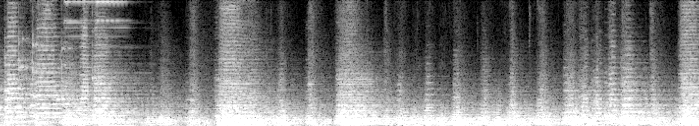
\includegraphics[width=0.9\textwidth]{specgram_classical.png}
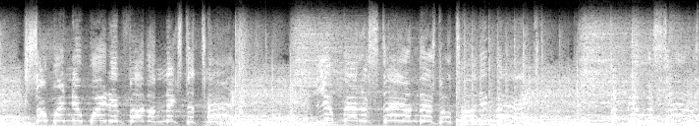
\includegraphics[width=0.9\textwidth]{specgram_metal.png}
\caption{Espectrograma de una canción `classical' (arriba) y `metal' (abajo).}
\label{fig:specgram}
\end{figure}

La amplitud puede estar en escala lineal o logarítmica (por ejemplo, decibeles).
Normalmente se escoge escala logarítmica, escala que usamos aquí.

Los espectrogramas son una representación muy usada para distintas tareas como
música, sonares, radares, procesamiento del habla, y en años recientes, para
identificar eventos en muestras de sonido como en \cite{audio_recognition}.

\section{Aprendizaje colectivo}

En el proyecto \textit{Is this Loss? Sistema de reconocimiento de objetos en
imágenes} ya se habló de las redes convolucionales por lo que aquí se omite su
discusión y procedemos a hablar de clasificadores colectivos.

El aprendizaje colectivo, en inglés \textit{ensemble learning}\footnote{Traducción
del término adoptada por los autores del presente escrito.}, es el proceso de usar
distintos modelos, ya sean clasificadores o expertos, generados y combinados
estratégicamente para lograr un mejor desempeño en tareas de predicción (clasificación
o regresión).

\section{Datos y preprocesamiento}

El dataset para el proyecto es \textsf{GTZAN Genre Collection}%
\footnote{\url{http://marsyasweb.appspot.com/download/data_sets/}}, que consiste de
una colección de 1000 clips de canciones con una duración de 30 segundos cada uno,
clasificados en 10 géneros musicales distintos: blues, classical, country, disco,
hiphop, jazz, metal, pop, reggae y rock, 100 clips por género.

Se obtuvo el espectrograma de estos clips, y estos espectrogramas (imágenes
\texttt{.png}) son los datos que se usaron para realizar una clasificación con
redes convolucionales.

Los espectrogramas obtenidos son arreglos de 3 dimensiones: tiempo, frecuencia
y amplitud. A la amplitud aplicamos logaritmo base 10 para tener una escala en
decibeles.

\section{Experimentación}

\section{Resultados}

\section{Conclusiones}

\begin{thebibliography}{9}
\bibitem{scholarpedia}
Ensemble Learning. (2009). Obtenido de
\url{http://www.scholarpedia.org/article/Ensemble_learning}

\bibitem{audio_recognition}
Phan, H., Hertel, L., Maass, M., \& Mertins, A. (2016).
Robust Audio Event Recognition with 1-Max Pooling Convolutional Neural Networks.
arXiv:1604.06338v2

\end{thebibliography}


\end{document}
